\documentclass[a4paper,10pt]{article}
\usepackage{graphicx}
\pagestyle{myheadings}
\markright{Fabien Perry, Camille Schnell, Lo\"ic Souverain \\ MPM2 ProjetMathsWinniie}

\begin{document}
  \begin{center}
  \textbf{\huge{Rapport Projet Maths}}
  \end{center}
  \section{Introduction}
    Le but de ce projet math est de coder plusieurs fonctions (en C++) afin de r\'esoudre l'\'equation de la Magn\'eto-Hydro-Dynamique mod\'elisant l'\'evolution d’un fluide conducteur dans un champ magn\'etique.
  \section{Contexte math\'ematiques}
    \begin{enumerate}
    \item
      Le syst\`eme d'\'equations de la Magn\'eto-Hydro-Dynamique (MHD) est :
    \begin{equation}
      \partial_t
      \left( \begin{array}{c}
      \rho \\
      \rho u \\
      Q \\
      B
      \end{array}
    \right)
    + \nabla .
    \left( \begin{array}{c}
      \rho u \\
      \rho u \otimes u + (p + \frac{B.B}{2})I - B \otimes B \\
      (Q + p + \frac{B.B}{2})u - (B.u)B \\
      u \otimes B - B \otimes u \\
      \end{array}
    \right)
    = 0,
    \end{equation}
    \begin{equation}
      Q = \rho e + \rho \frac{u.u}{2} + \frac{B.B}{2}
    \end{equation}
    \begin{equation}
      p = P(\rho,e) = (\gamma - 1)\rho e, \gamma > 1.
    \end{equation} \\


    \item
     En utilisant la m\'ethode propos\'ee en 2002, ce syst\`eme devient : \\
     \begin{center}
       \begin{math}
         \partial_t
         \left( \begin{array}{c}
         \rho \\
         \rho u \\
         Q \\
         B \\
         \psi
         \end{array}
       \right)
       + \nabla .
       \left( \begin{array}{c}
         \rho u \\
         \rho u \otimes u + (p + \frac{B.B}{2})I - B \otimes B \\
         (Q + p + \frac{B.B}{2})u - (B.u)B \\
         u \otimes B - B \otimes u + \psi I\\
         c^2_h B
         \end{array}
       \right)
       = \left( \begin{array}{c}
         0 \\
         0 \\
         0 \\
         0 \\
         0
         \end{array}
        \right)
      \end{math}
     \end{center}

    \item
    Le syst\`eme de la MHD sous la forme d'une \'equation conservative donne : \\
    \begin{center}
      \begin{math}
        \frac{\partial}{\partial t}W + \sum\limits_{i=1}^d \frac{\partial}{\partial x_i}F^i(W) = 0.
      \end{math}
    \end{center}

    En consid\'erant :
    \begin{math}
      \partial\star = \frac{\partial}{\partial x_\star}
    \end{math}
     et
     \begin{math}
       \partial_iF^i(W) = \sum\limits_{i=1}^d\frac{\partial}{\partial x_i}F^i(W).
     \end{math} \\
     On obtient l'\'equation :
     \begin{math}
       \partial_tW+\partial_iF^i(W) = 0.
     \end{math}
     \\\\
     Le vecteur de variables conservatives \textbf{W} est :
     \begin{math}
       \textbf{W} =\left(\rho, \rho \textbf{u}, Q, \textbf{B}\right)^T
     \end{math}
     \\
     Le vecteur de variables primitives \textbf{Y} est :
     \begin{math}
       \textbf{Y} =\left(\rho, \textbf{u}, \rho, \textbf{B}\right)^T
     \end{math}

    \item
      Les fonctions \textit{conservatives(real* Y, real* W)} et \textit{primitives(real* Y, real* W)} permettent de calculer les variables conservatives \`a partir des variables primitives ou inversement. On applique la formule pour obtenir \textbf{p} ou \textbf{Q}.
    \item
      La fonction \textit{flux(real* W, real* vn, real* flux)} utilise la formule pour calculer le flux suivant \textbf{W} et \textbf{n}, \`a partir du vecteur des variables conservatives et d'un vecteur n de l'espace. On utilise d'abord la fonction \textit{primitives} pour obtenir le vecteur des variables primitives et pouvoir ensuite appliquer la formule.
   \end{enumerate}
 \section{Autre}
   \begin{enumerate}
     \item
       La fonction \textit{Ref2Phy(real* x, real *y, real *z, real *t)} permet d'obtenir les coordonn\'ees \textit{(z,t)} appartenant \`a [XMIN,XMAX]*[YMIN,YMAX], \`a partir de coordonn\'ees \textit{(x,y)} appartenant \`a \begin{math} [0,1]^2 \end{math}. \\
       Pour faire cela, il ne faut pas oublier de centrer la valeur en z\'ero : \\
       \begin{math}
         z = (x - 0.5) * (X_{MAX} - X_{MIN}) + \frac{(X_{MIN} + X_{MAX})}{2}. \\
         t = (y - 0.5) * (Y_{MAX} - Y_{MIN}) + \frac{(Y_{MIN} + Y_{MAX})}{2}. \\
       \end{math}
     \item
      \begin{enumerate}
        \item
        \textun{Structure du tableau :} \\
        Avant de commencer \`a remplir le tableau,il a fallu comprendre de quel tableau il s'agissait, et ce qu'il contenait : \textbf{w} est un (real *w), c'est-\`a- dire un tableau de r\'eels \`a une dimension. Il s'agit en fait d'un tableau \`a plusieurs dimensions qui a \'et\'e lin\'earis\'e. \\
        Il y a donc des cellules de coordonn\'ees \textit{(x,y)}, et pour chacune de ces cellules, on a 9 caract\'eristiques \begin{math}(\rho, u1, p, u2, u3, B1, B2, B3, \psi)\end{math}.\\
        Le tableau a \'et\'e lin\'earis\'e de la mani\`ere suivante : dans w[k*\_NXTRANSBLOCK * \_NYTRANSBLOCK + j * \_NXTRANSBLOCK + i], se trouve la composante \textit{k} de la cellule \texit{(i,j)}. \\
        Avec \_NXTRANSBLOCK-1 la coordonn\'ee maximale en x, \_NYTRANSBLOCK-1 la coordonn\'ee maximale en y, et \_M le nombre de composantes d'une cellule \textit{(x,y)}. Ces valeurs sont fix\'ees \`a (128,128,9) dans le programme. \\\\
        Le choix de la m\'ethode de linéarisation de w qui consiste \`a dire que \textit{"dans w[k*\_NXTRANSBLOCK*\_NYTRANSBLOCK + j * \_NXTRANSBLOCK + i], se trouve la composante k de la cellule (i,j)"}
        a des d\'efauts par rapport \`a une impl\'ementation du type \textit{"dans w[i*\_NXTRANSBLOCK*\_M + j*\_M + k], on trouve la composante k de [i,j]"}. \\
        Premi\`erement, c'est assez contre-intuitif, de plus ce n'est pas performant : \\
        \`A chaque \'etape, on a des formules qui nous donnent les composantes d'une cellule \textit{[x,y]} et on les stocke dans \textbf{w}. Dans la deuxi\`eme m\'ethode, on doit remplir les cases du tableau qui sont successives, alors que dans la premi\`ere m\'ethode, on doit acc\'eder \`a des cases tr\`es \'eloign\'ees du tableau. Or, lorsque l'on acc\`ede \`a une case d'un tableau, plusieurs cases successives sont charg\'ees en m\'emoire par souci d'optimisation. La deux\`eme m\'ethode permettrait donc de profiter de cette optimisation.
        \item
        Algorithme. \\
        Le principe du programme est le suivant : \\
        Pour chaque cellule \textit{(i,j)}, on calcule un couple \begin{math}\textit{(i2,j2)} = (\frac{i}{\_NXTRANSBLOCK}, \frac{j}{\_NYTRANSBLOCK}).\end{math} \\
        On applique ensuite \textit{Ref2PhysMap} sur \textit{i2} et\textit{j2} (qui sont dans \begin{math}[0,1]^2\end{math}), pour obtenir \textit{(x,y)} dans [xmin, xmax]*[ymin, ymax]. \\
        On appelle ensuite \textit{Wexact} sur \textit{(x,y)} et on stocke le r\'esultat dans 'wtmp'. \\
        On affecte finalement les valeurs de 'wtmp' dans 'w' gr\^ace \`a la formule de lin\'earisation du tableau vue dans la partie 1.
        \item
        R\'esultat de gmsh apr\`es l'initialisation du tableau 2D : \\\\
        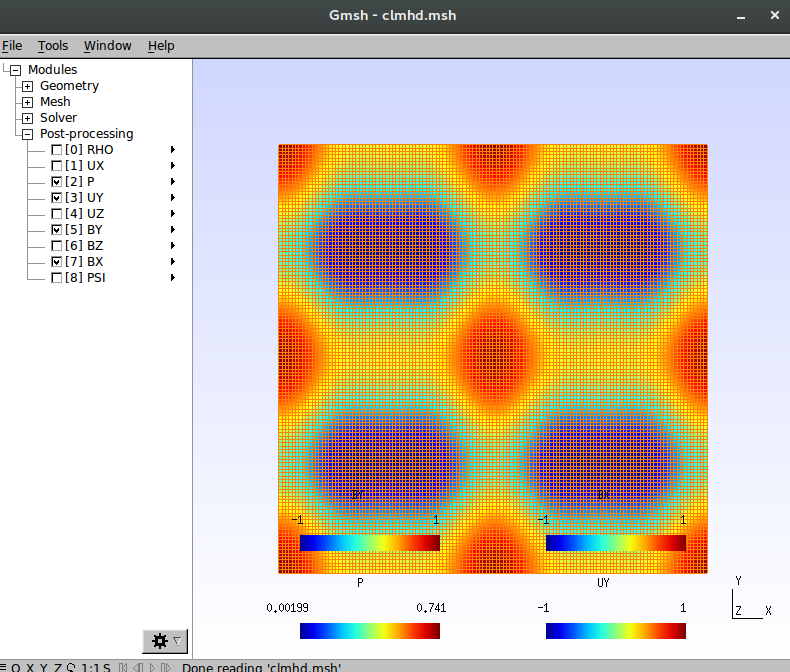
\includegraphics[scale=0.5]{init.png}
      \end{enumerate} \newpage
     \item
      La fonction \textit{TimesStepCPU1D(real Wn1[\_NXTRANSBLOCK*\_NYTRANSBLOCK*\_M], real* dtt)} r\'ecup\`ere les variables conservatives \`a chaque it\'eration n, afin de calculer la valeur \`a l'it\'eration n + 1 en appliquant la formule. \\
      R\'esultat de GnuPlot apr\`es ex\'ecution du programme en 1D : \\\\
      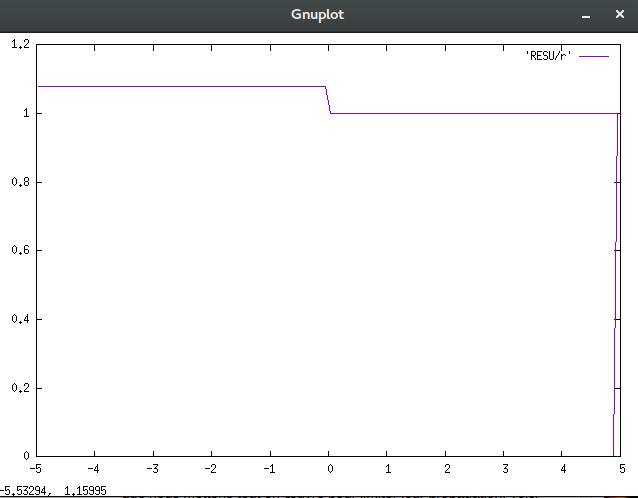
\includegraphics[scale = 0.5]{ts1d.png} \\
     \item
      La fonction \textit{TimesStepCPU2D(real Wn1[\_NXTRANSBLOCK*\_NYTRANSBLOCK*\_M], real* dtt)} ressemble \`a la fonction pr\'ec\'edente, sauf que l'on s'int\'eresse \'egalement aux cases au-dessus et en-dessous.
     \end{enumerate}
\end{document}
